\documentclass[aspectratio=169]{beamer}

\usepackage[utf8]{inputenc}
\usepackage[T1]{fontenc}
\usetheme{plam-2026}

% PLAM-2026 theme on a white canvas: light colours, vector Percona Live logo,
% white arrow interior. \input after \usetheme{plam-2026}.

% light variant: white canvas, dark text (plam-2026 is dark by default, and
% \usecolortheme{percona-2026} is a no-op here since the theme already loaded it)
\setbeamercolor*{normal text}{fg=percona-2026black,bg=white}
\setbeamercolor*{background canvas}{bg=white}
\setbeamercolor*{frametitle}{fg=percona-2026black}
\setbeamercolor*{itemize item}{fg=percona-2026black}
\setbeamercolor*{itemize subitem}{fg=percona-2026black}
\setbeamercolor*{itemize subsubitem}{fg=percona-2026black}
\setbeamercolor*{itemize/enumerate body}{fg=percona-2026black}
\setbeamercolor*{itemize/enumerate subbody}{fg=percona-2026black}
\setbeamercolor*{itemize/enumerate subsubbody}{fg=percona-2026black}
\setbeamercolor*{enumerate item}{fg=percona-2026black}
\setbeamercolor*{enumerate subitem}{fg=percona-2026black}

% theme loads moreverb but never uses it, drop its listing envs so minted can define its own
\makeatletter
\expandafter\let\csname listing\endcsname\@undefined
\expandafter\let\csname endlisting\endcsname\@undefined
\expandafter\let\csname listing*\endcsname\@undefined
\expandafter\let\csname endlisting*\endcsname\@undefined
\makeatother
\usepackage{minted}
\usetikzlibrary{calc}

\graphicspath{{./theme/images/}}

\pgfplotsset{compat=1.18}

\setminted{fontsize=\footnotesize,style=default}

% same as the plam-2026 frametitle template, but title box ends before the
% triangle decoration (0.85\paperwidth) so long titles wrap instead of overflowing,
% and the arrow's inner triangle is white to match the canvas
\setbeamertemplate{frametitle}{
  \begin{textblock*}{\paperwidth}(0pt,0pt)
    \tikz[remember picture,overlay] {%
      \draw[fill=percona-2026blue,percona-2026blue] (0\paperwidth,-0.76\paperheight) -- (0.07\paperwidth,-1\paperheight) -- (0\paperwidth,-1\paperheight) -- cycle;
    }
  \end{textblock*}

  \begin{textblock*}{\paperwidth}(0.85\paperwidth,0\paperheight)
    {
\includegraphics[width=0.18\paperwidth,keepaspectratio]{plam2026_slide.png}}
  \end{textblock*}

  \begin{tikzpicture}[overlay, remember picture]
    \begin{scope}[shift={(current page.north west)}]
      \draw[fill=percona-2026blue,percona-2026blue] (0.021\paperwidth,-0.128\paperheight) -- (0.054\paperwidth,-0.160\paperheight) -- (0.021\paperwidth,-0.191\paperheight) -- cycle;
      \draw[fill=white,white] (0.025\paperwidth,-0.137\paperheight) -- (0.048\paperwidth,-0.160\paperheight) -- (0.025\paperwidth,-0.182\paperheight) -- cycle;
    \end{scope}
  \end{tikzpicture}

  \begin{textblock*}{0.78\paperwidth}(0.06\paperwidth,0.12\paperheight)
    \begin{beamercolorbox}[left, wd=0.78\paperwidth]{frametitle}
      \usebeamerfont{title in head/foot}\insertframetitle
    \end{beamercolorbox}%
  \end{textblock*}
}

% same as the percona-2026 title page template, but with the vector logo
% instead of the low-res png
\setbeamertemplate{title page}{
  \begin{textblock*}{\paperwidth}(0\paperwidth,0\paperheight)
    {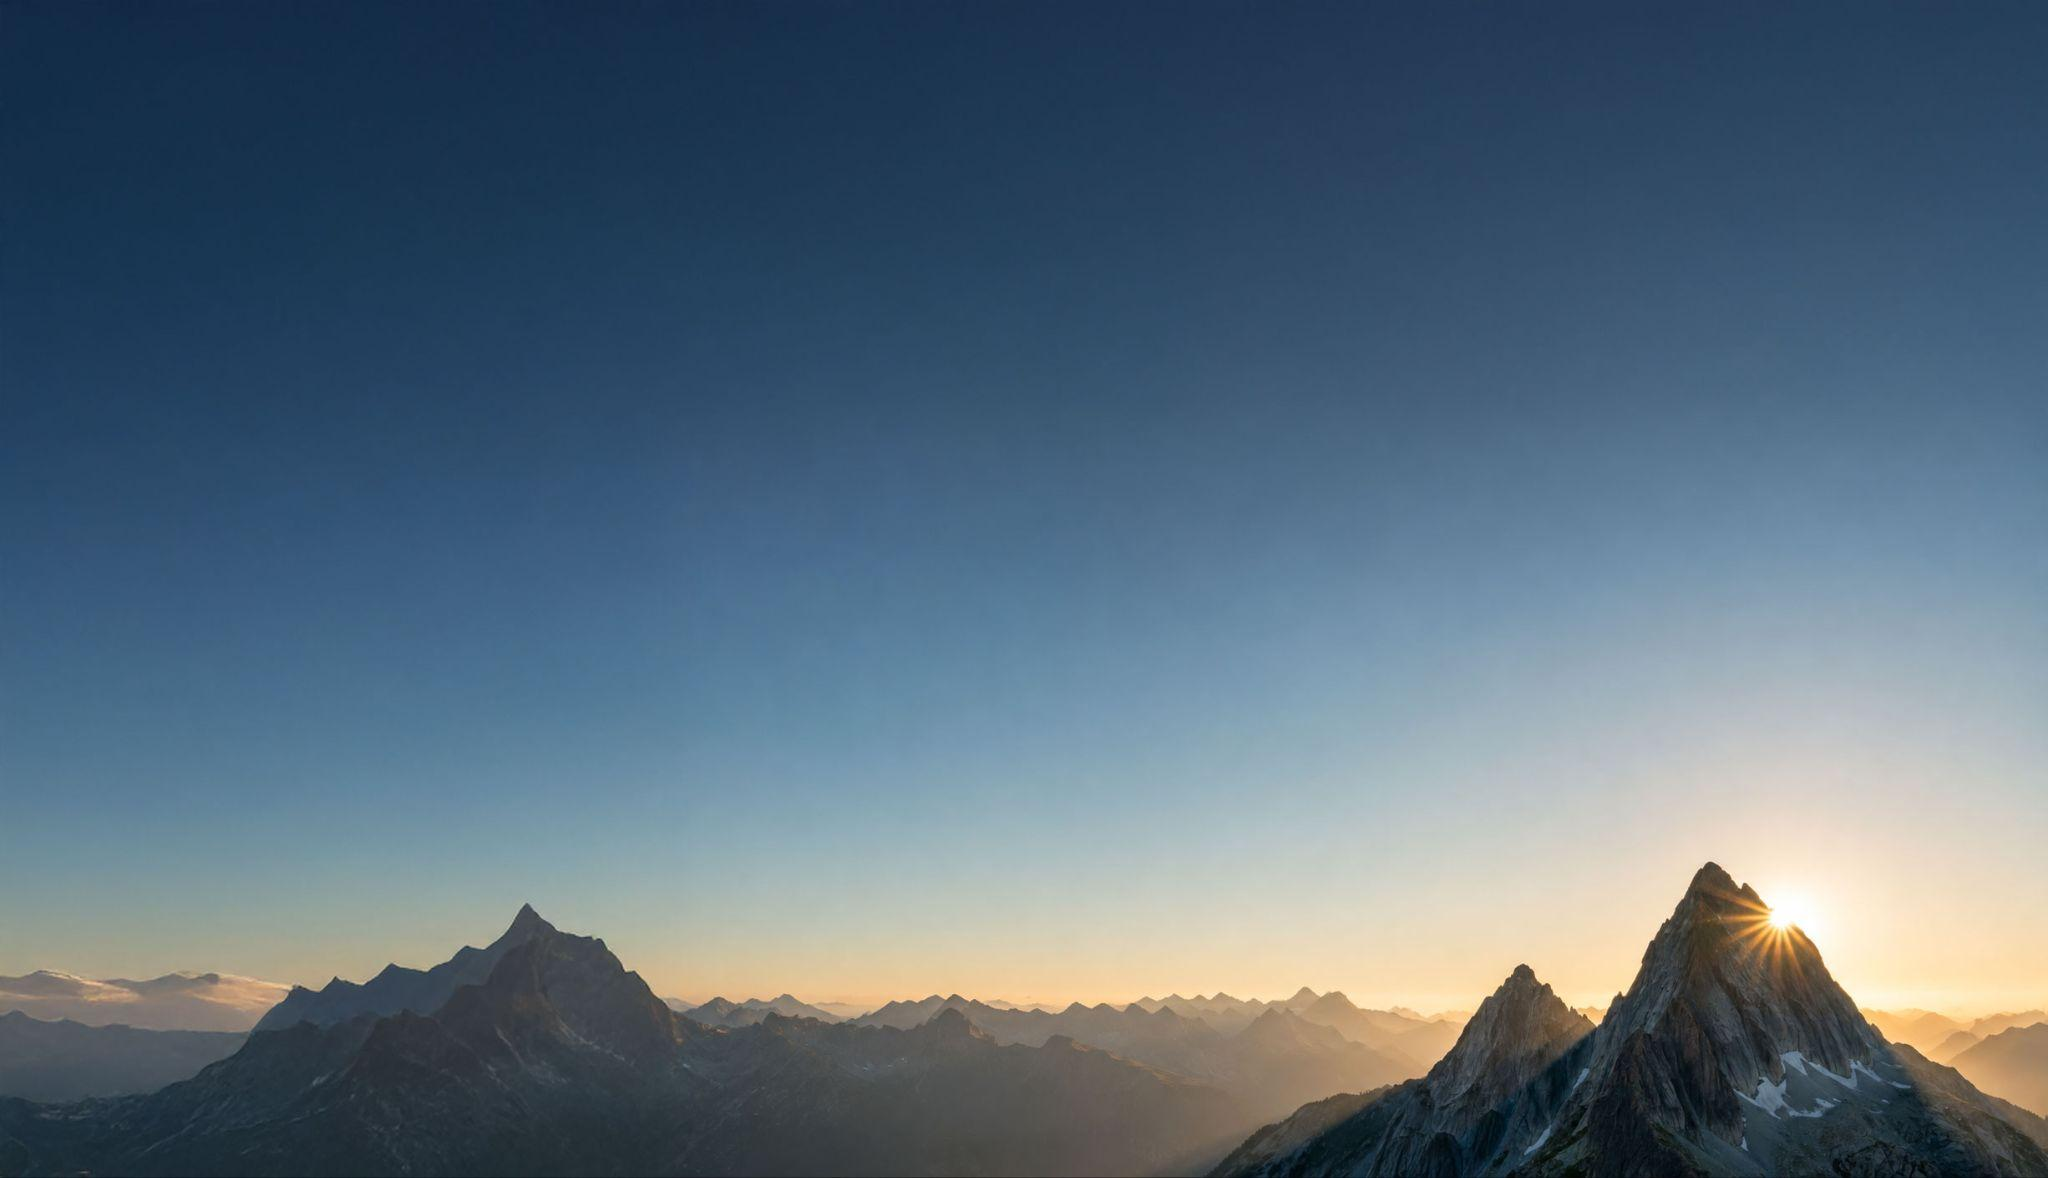
\includegraphics[width=\paperwidth,keepaspectratio]{plam2026_title.jpg}}
  \end{textblock*}

  \begin{textblock*}{\paperwidth}(0\paperwidth,0\paperheight)
  \begin{tikzpicture}[overlay, remember picture]
    \begin{scope}[shift={(current page.north west)}]
      \draw[fill=percona-2026black,percona-2026black] (0.078\paperwidth,0\paperheight) -- (\paperwidth,0\paperheight) -- (0.675\paperwidth,-1\paperheight) -- (0\paperwidth,-1\paperheight) -- (0\paperwidth,-0.245\paperheight) -- cycle;
      \draw[fill=percona-2026yellow,percona-2026yellow] (0\paperwidth,0\paperheight) -- (0.078\paperwidth,0\paperheight) -- (0\paperwidth,-0.245\paperheight) -- cycle;

      \draw[fill=percona-2026blue,percona-2026blue] (0.341\paperwidth,-0.666\paperheight) -- (0.374\paperwidth,-0.698\paperheight) -- (0.341\paperwidth,-0.729\paperheight) -- cycle;
      \draw[fill=percona-2026black,percona-2026black] (0.345\paperwidth,-0.675\paperheight) -- (0.368\paperwidth,-0.698\paperheight) -- (0.345\paperwidth,-0.720\paperheight) -- cycle;
    \end{scope}
  \end{tikzpicture}
  \end{textblock*}

  \begin{textblock*}{0.48\paperwidth}(0.32\paperwidth,0.125\paperheight)
    \begin{beamercolorbox}{title page header}
      \usebeamerfont{title}\inserttitle\hfill%
    \end{beamercolorbox}%
  \end{textblock*}

  \begin{textblock*}{0.353\paperwidth}(0.38\paperwidth,0.64\paperheight)
    \begin{beamercolorbox}{author}
      {\usebeamerfont{author}\insertauthor}\hfill\par\usebeamerfont{institute}\insertinstitute\hfill\par\usebeamerfont{date}\insertdate\hfill%
    \end{beamercolorbox}%
  \end{textblock*}

  \begin{textblock*}{\paperwidth}(0.06\paperwidth,0.222\paperheight)
    {\includegraphics[width=0.222\paperwidth,keepaspectratio]{perconalive_light.pdf}}
  \end{textblock*}
}

% theme footline logo is white text, invisible on white canvas: use the dark variant instead
\setbeamertemplate{footline}{
  \ifnum \insertpagenumber=1
  \else
    \begin{textblock*}{\paperwidth}(0.85\paperwidth,0.7\paperheight)
      {\includegraphics[width=0.1\paperwidth,keepaspectratio]{perconalive.pdf}}
    \end{textblock*}

    \begin{textblock*}{\paperwidth}(0.025\paperwidth,0.95\paperheight)
      \begin{beamercolorbox}{framenumber}
        \usebeamerfont{framenumber}\insertpagenumber%
      \end{beamercolorbox}%
    \end{textblock*}

    \begin{textblock*}{\paperwidth}(0.85\paperwidth,0.95\paperheight)
      \begin{beamercolorbox}{copyright}
        \usebeamerfont{copyright}\textcopyright~\the\year~Percona
      \end{beamercolorbox}%
    \end{textblock*}

    \vskip0.3in%
  \fi
}

% Template \tyslide needs social icon images missing from the repo, so build the slide by hand
\newcommand{\thankyouslide}{
{
\usebackgroundtemplate{
\includegraphics[width=\paperwidth,keepaspectratio]{ty_bg.jpg}}
\setbeamertemplate{footline}{}
\begin{frame}[plain]
  \begin{textblock*}{\paperwidth}(0pt,0pt)
    \tikz[remember picture,overlay] {%
      \draw[fill=percona-2026blue,percona-2026blue] (0.922\paperwidth,0\paperheight) -- (1\paperwidth,0\paperheight) -- (\paperwidth,-0.245\paperheight) -- cycle;
    }
  \end{textblock*}

  \begin{textblock*}{\paperwidth}(0pt,0.38\paperheight)
    \centering
    {\usebeamerfont{title}\color{percona-2026white}Thank you!}
  \end{textblock*}

  \begin{textblock*}{\paperwidth}(0.790\paperwidth,0.87\paperheight)
    {
\includegraphics[width=0.18\paperwidth,keepaspectratio]{percona_one_color_light.png}}
  \end{textblock*}
\end{frame}
}
}


\newcommand{\imageslide}[2]{
  \begin{frame}{#1}
    \centering
    \includegraphics[height=0.65\textheight]{#2}
  \end{frame}
}

% steps.png regions (pixel coords, 1536x1024, origin top left) covering each
% step's badge, label and arrow, faded to grey out already discussed steps
\newlength{\stepsW}
\newlength{\stepspx}
\newcommand{\greyrect}[4]{\fill[white,opacity=0.8] (#1,#2) rectangle (#3,#4);}
\newcommand{\defgrey}[2]{\expandafter\def\csname greystep#1\endcsname{#2}}
\defgrey{1}{\greyrect{235}{180}{470}{250}\greyrect{210}{266}{495}{284}}
\defgrey{2}{\greyrect{798}{138}{1110}{196}\greyrect{772}{201}{1165}{219}}
\defgrey{3}{\greyrect{802}{265}{1150}{322}\greyrect{772}{243}{1165}{261}}
\defgrey{4}{\greyrect{383}{532}{605}{590}\greyrect{591}{425}{609}{690}}
\defgrey{5}{\greyrect{128}{683}{365}{745}\greyrect{86}{483}{104}{782}\greyrect{86}{761}{487}{779}}
\defgrey{6}{\greyrect{703}{528}{920}{590}\greyrect{674}{425}{692}{690}}
\defgrey{7}{\greyrect{800}{362}{1100}{422}\greyrect{772}{341}{1165}{359}}
\defgrey{8}{\greyrect{920}{648}{1210}{732}\greyrect{1213}{425}{1231}{762}\greyrect{780}{741}{1231}{759}\greyrect{1261}{425}{1279}{800}\greyrect{780}{781}{1281}{799}}
\defgrey{9}{\greyrect{1312}{548}{1530}{637}\greyrect{780}{801}{1352}{819}\greyrect{1331}{425}{1349}{818}}

% #1: last step to grey out (all steps up to and including it), 0 for none
\newcommand{\stepsslide}[1]{
  \begin{frame}{It's just communication}
    \begin{textblock*}{\paperwidth}(0pt,0.2\paperheight)
      \centering
      \setlength{\stepsW}{1.185\paperheight}
      \setlength{\stepspx}{\stepsW}
      \divide\stepspx by 1536
      \begin{tikzpicture}
        \node[anchor=south west,inner sep=0] (img) {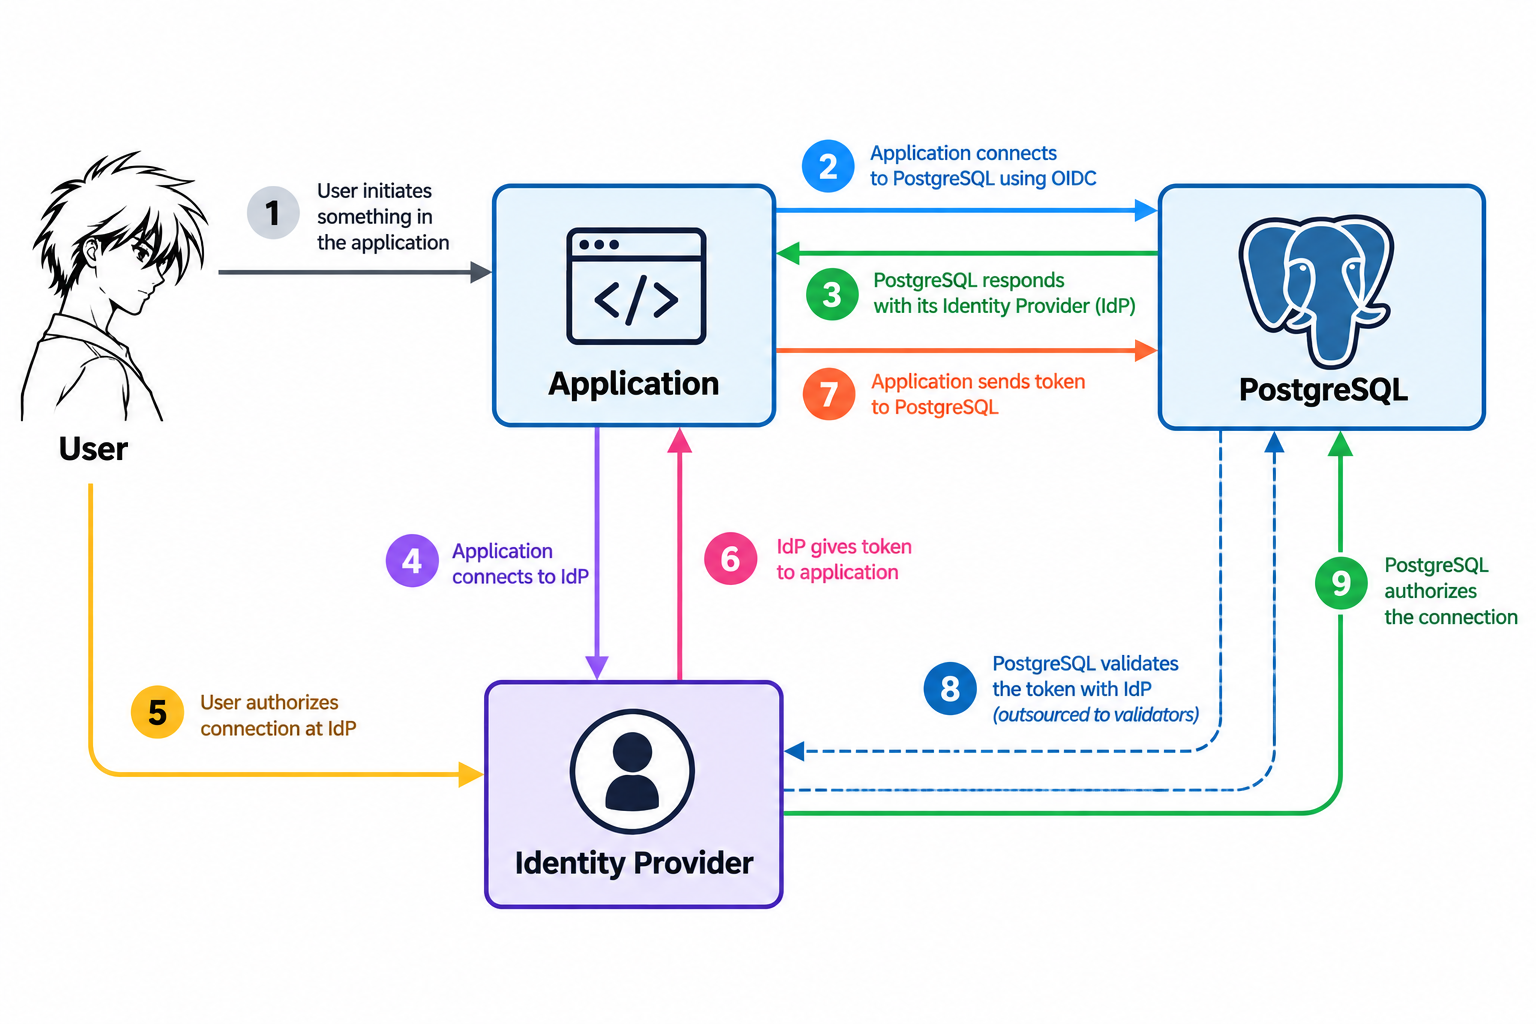
\includegraphics[width=\stepsW]{steps.png}};
        \begin{scope}[shift={(img.north west)},x=\stepspx,y=-\stepspx]
          \ifnum#1>0 \foreach \s in {1,...,#1} {\csname greystep\s\endcsname}\fi
        \end{scope}
      \end{tikzpicture}
    \end{textblock*}
  \end{frame}
}

\title{Following the Token: A Practical Guide to OAuth in PostgreSQL}
\author{Zsolt Parragi}
\institute{Percona}
\date{Percona Live Amsterdam 2026}

\begin{document}

\begin{frame}[plain]
  \titlepage
\end{frame}

\begin{frame}{Who am I?}
  \begin{itemize}
    \item Zsolt Parragi
    \item Software developer at Percona for 9 years
    \item Author of \ttf{pg\_oidc\_validator}
    \item Active contributor in PostgreSQL OAuth development
  \end{itemize}
\end{frame}

\begin{frame}{What's OAuth/OIDC?}
  \begin{itemize}
    \item Passwordless authentication
    \item Centralized identity management
    \item Seamless integration with enterprise identity providers
    \item Simple to use
  \end{itemize}
\end{frame}

\begin{frame}{Simple?}
  \begin{textblock*}{\paperwidth}(0pt,0.2\paperheight)
    \centering
    \includegraphics[height=0.79\paperheight]{mermaid.png}
  \end{textblock*}
\end{frame}

\imageslide{Even simpler?}{even-simpler.png}

\imageslide{When something goes wrong}{the-plan.png}

\begin{frame}{OIDC requires extensions}
  \begin{itemize}
    \item Token validation is not in core
    \item There are already multiple external validators
    \item There is at least one that doesn't properly validate the token
  \end{itemize}
\end{frame}

\begin{frame}[fragile]{A FATAL error is normal}
  \begin{columns}[T]
    \begin{column}{0.58\textwidth}
      \begin{itemize}
        \item Fixed in PostgreSQL 19
        \item Log spam for every connection using OAuthBearer discovery:
      \end{itemize}

\begin{minted}[xleftmargin=\leftmargini]{text}
FATAL:  OAuth bearer authentication
        failed for user "testuser"
\end{minted}

      \begin{itemize}
        \item Also displayed for real errors, but then there is a \ttf{WARNING} before it
      \end{itemize}
    \end{column}
    \begin{column}{0.4\textwidth}
      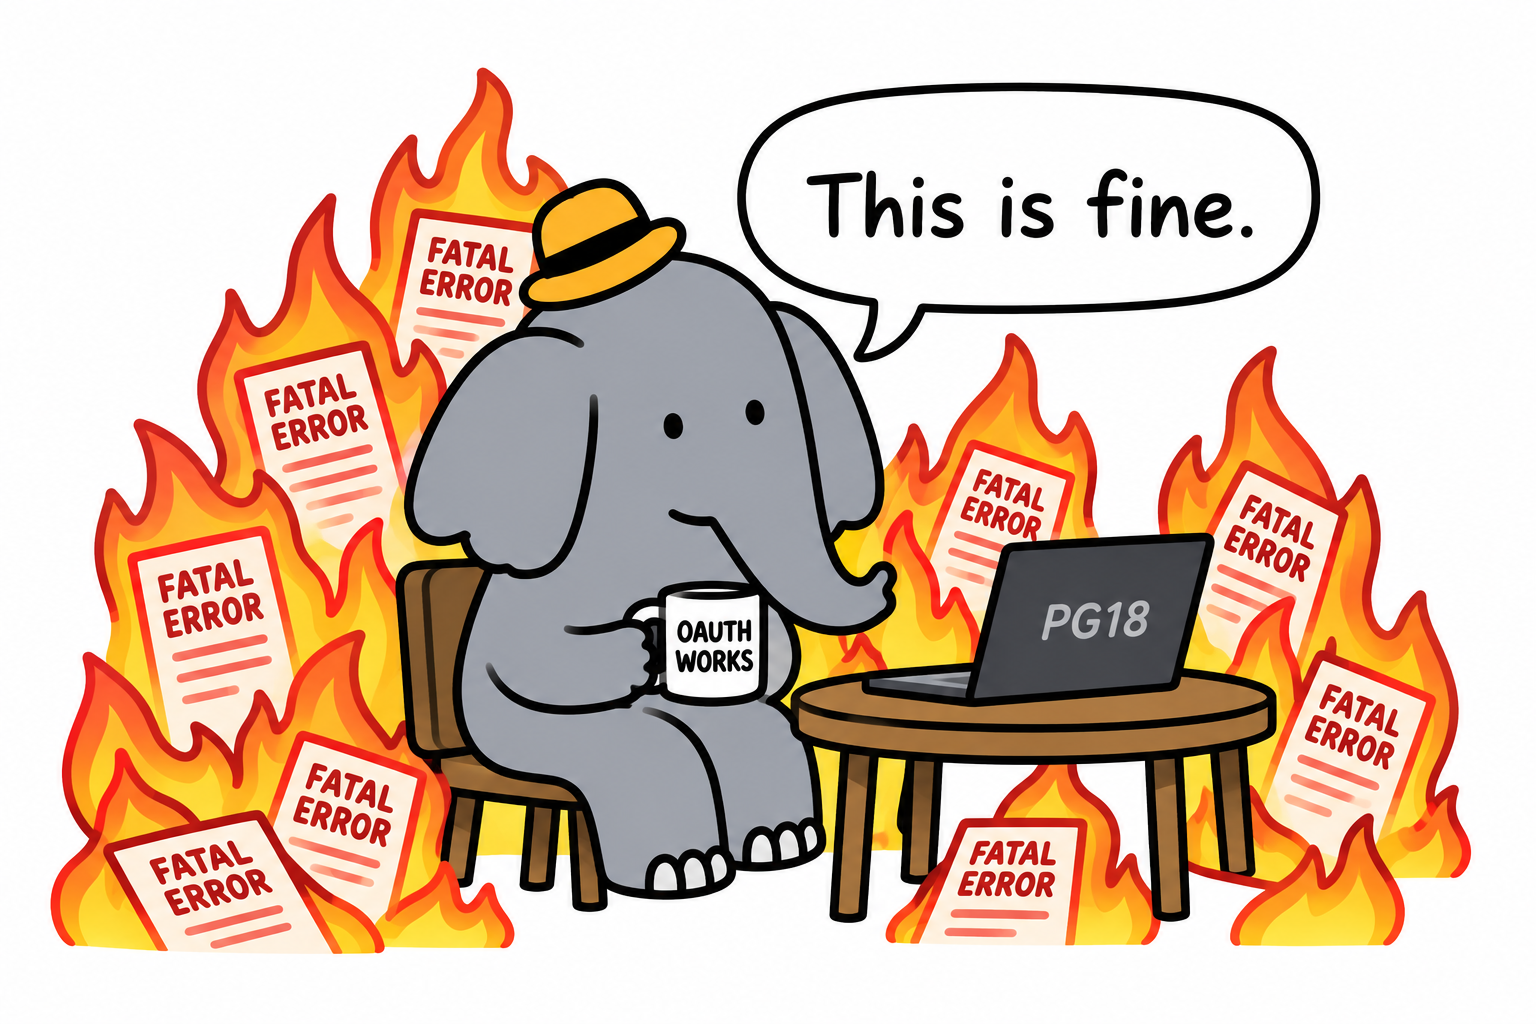
\includegraphics[width=\textwidth]{oauth-fatal.png}
    \end{column}
  \end{columns}
\end{frame}

\stepsslide{0}

\begin{frame}{HBA issues}
  \begin{itemize}
    \item \ttf{pg\_hba.conf} uses the first matching (ip, username, database name) rule
    \item No easy migration path with a login method choice
    \item No support for multiple OIDC providers for the same database
    \item If the first rule matches ALL connections to OIDC, good luck!
  \end{itemize}
\end{frame}

\stepsslide{2}

\begin{frame}{Identity provider mismatch}
  \begin{itemize}
    \item Both the server and the client have to use the exact same canonical URL
    \item This mainly prevents malicious servers from extracting tokens
    \item Centralized authentication: you have to think about the server attacking the users!
  \end{itemize}
\end{frame}

\stepsslide{3}

\begin{frame}{User token verification}
  \begin{itemize}
    \item A good\footnote{Not all identity providers are good} identity provider displays a detailed auth screen:
    \begin{itemize}
      \item name of the client application
      \item requested scopes
      \item any additional details/warnings added by the client application
    \end{itemize}
    \item Centralized authentication: you have to think about the server attacking the users!
    \item But also man in the middle and many other threats
  \end{itemize}
\end{frame}

\stepsslide{5}

\begin{frame}{Authorization errors}
  \begin{itemize}
    \item Does the role returned by the validator exist in PostgreSQL?
    \item Does it have a proper \ttf{pg\_ident.conf} mapping?
    \item Does the role pass the usual requirements of connecting to the database?
  \end{itemize}
\end{frame}

\stepsslide{7}

\begin{frame}{Validating the token}
  \begin{itemize}
    \item Exact mechanism is up to the validator
    \begin{itemize}
      \item a direct introspection endpoint
      \item validating the cryptographic signature of the token
    \end{itemize}
    \item Required claims/validity have to match
  \end{itemize}
\end{frame}

\begin{frame}{Introspection endpoint}
  \begin{itemize}
    \item The token is sent as-is to the IdP
    \item IdP answers if this is a valid token issued by it
    \item IdP also answers token details (permissions)
    \item Validator checks this against the PostgreSQL configuration
    \item Every backend has to connect to the IdP
    \item Token revocation is immediate
  \end{itemize}
\end{frame}

\begin{frame}{JWKS signature}
  \begin{itemize}
    \item Validator retrieves the public keys of the IdP
    \begin{itemize}
    \item Usually\footnote{Except some providers} can be cached for a long time
    \end{itemize}
    \item Validator verifies the signature against the public key
    \item No revocation: issued tokens remain valid
    \item Validator verifies token content:
    \begin{itemize}
      \item issuer URL
      \item scopes
      \item expiry time
      \item audience
      \item other claims
    \end{itemize}
  \end{itemize}
\end{frame}

\begin{frame}{Expired tokens}
  \begin{itemize}
    \item OIDC has a concept of token refresh
    \item PostgreSQL doesn't know about refresh tokens
    \item Validity is only checked at connection time
    \item Applications/clients have to make sure to refresh tokens as needed
  \end{itemize}
\end{frame}

\thankyouslide

\end{document}
